\documentclass[11pt,a4paper]{article}

\usepackage[margin=2.2cm]{geometry}
\usepackage[T1]{fontenc}
\usepackage{lmodern}
\usepackage{microtype}
\usepackage{xcolor}
\usepackage{booktabs}
\usepackage{array}
\usepackage{enumitem}
\usepackage{listings}
\usepackage{fancyhdr}
\usepackage{tikz}
\usetikzlibrary{arrows.meta,positioning,shapes.geometric,fit,calc}
\usepackage[hidelinks]{hyperref}

\definecolor{accent}{HTML}{1F5FA8}
\definecolor{good}{HTML}{2E7D32}
\definecolor{bad}{HTML}{C62828}
\definecolor{warn}{HTML}{EF6C00}
\definecolor{codebg}{HTML}{F5F7FA}
\definecolor{keyword}{HTML}{8A2BE2}
\definecolor{comment}{HTML}{5F7F5F}

\lstset{
  basicstyle=\ttfamily\small,
  backgroundcolor=\color{codebg},
  keywordstyle=\color{keyword}\bfseries,
  commentstyle=\color{comment}\itshape,
  language=Java,
  frame=single,
  rulecolor=\color{black!15},
  breaklines=true,
  columns=fullflexible,
  keepspaces=true,
  showstringspaces=false,
  aboveskip=0.8em,
  belowskip=0.6em
}

\newcommand{\code}[1]{\texttt{\small #1}}

\renewcommand{\arraystretch}{1.25}
\setlist{itemsep=2pt,topsep=4pt}
\setlength{\parindent}{0pt}
\setlength{\parskip}{0.55em}

\pagestyle{fancy}
\fancyhf{}
\lhead{AgentGate -- Day 2 short note}
\rhead{Policy Service}
\cfoot{\thepage}
\renewcommand{\headrulewidth}{0.3pt}

% ---- TikZ styles
\tikzset{
  box/.style={draw=accent!70!black, fill=accent!8, rounded corners=3pt, align=center,
              minimum height=8mm, inner sep=4pt, font=\small},
  okbox/.style={box, draw=good!70!black, fill=good!10},
  badbox/.style={box, draw=bad!70!black, fill=bad!8},
  warnbox/.style={box, draw=warn!80!black, fill=warn!10},
  dbox/.style={draw=warn!80!black, fill=warn!10, diamond, aspect=2.4, align=center,
               inner sep=1pt, font=\small},
  arr/.style={-{Stealth[length=2.4mm]}, thick, draw=black!70},
  lbl/.style={font=\scriptsize, fill=white, inner sep=1.5pt}
}

\begin{document}

\begin{center}
  {\Huge\bfseries\color{accent} AgentGate}\\[0.4em]
  {\Large Day 2 Short Note: Validation Errors, Unit Tests, Cache}\\[0.5em]
  {\normalsize Tuesday, 27 October 2026 \quad|\quad Week 1 finished}
\end{center}
\vspace{0.2em}
\hrule
\vspace{0.6em}

% ------------------------------------------------------------------
\section*{Summary}

\begin{tabular}{@{}p{3.4cm}p{12.4cm}@{}}
\toprule
\textbf{Done today} & \code{GlobalExceptionHandler}, 5 Mockito unit tests, Caffeine cache with eviction. \\
\textbf{Result} & Week 1 is complete, five days before the 1 November deadline. \\
\textbf{Proof} & Invalid request returns a clean \code{application/problem+json} 400. \code{Tests run: 5, Failures: 0}. Cache measured: repeated checks add no database query, and a new rule clears the cache. \\
\textbf{Next} & Week 2: Auth Service (OAuth2, token exchange) and Gateway. Starts 2 November. \\
\bottomrule
\end{tabular}

% ------------------------------------------------------------------
\section{Validation errors: \texttt{@Valid} and the exception handler}

\code{@Valid} means: \emph{before my method runs, check the incoming object against the
rules written on its fields}. The rules (\code{@NotBlank}, \code{@NotNull}) do nothing
without it.

\begin{center}
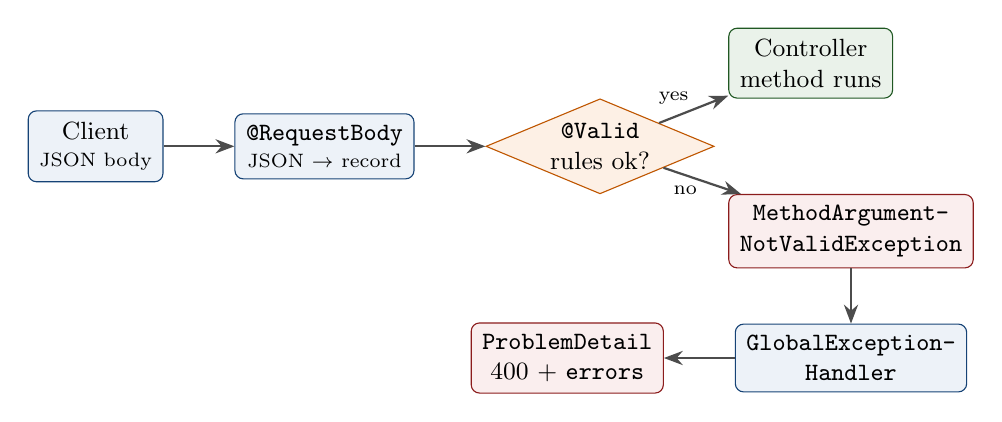
\begin{tikzpicture}[node distance=7mm and 9mm]
  \node[box] (client) {Client\\[-1pt]{\scriptsize JSON body}};
  \node[box, right=of client] (conv) {\code{@RequestBody}\\[-1pt]{\scriptsize JSON $\rightarrow$ record}};
  \node[dbox, right=of conv] (valid) {\code{@Valid}\\rules ok?};
  \node[okbox, above right=3mm and 9mm of valid] (ok) {Controller\\method runs};
  \node[badbox, below right=3mm and 9mm of valid] (ex) {\code{MethodArgument-}\\\code{NotValidException}};
  \node[box, below=of ex] (adv) {\code{GlobalException-}\\\code{Handler}};
  \node[badbox, left=of adv] (pd) {\code{ProblemDetail}\\400 + \code{errors}};

  \draw[arr] (client) -- (conv);
  \draw[arr] (conv) -- (valid);
  \draw[arr] (valid) -- node[lbl,above left] {yes} (ok);
  \draw[arr] (valid) -- node[lbl,below left] {no} (ex);
  \draw[arr] (ex) -- (adv);
  \draw[arr] (adv) -- (pd);
\end{tikzpicture}
\end{center}

\begin{lstlisting}
@RestControllerAdvice                       // watches ALL controllers
public class GlobalExceptionHandler {
    @ExceptionHandler(MethodArgumentNotValidException.class)   // handles this exception
    public ProblemDetail handleValidation(MethodArgumentNotValidException ex) {
        Map<String, String> errors = new LinkedHashMap<>();
        ex.getBindingResult().getFieldErrors()
          .forEach(e -> errors.put(e.getField(), e.getDefaultMessage()));
        ProblemDetail p = ProblemDetail.forStatusAndDetail(HttpStatus.BAD_REQUEST,
                                                           "One or more fields are invalid");
        p.setTitle("Validation failed");
        p.setProperty("errors", errors);
        return p;
    }
}
\end{lstlisting}

\textbf{Real response} (blank \code{tenantId} and \code{agentId}, no \code{effect}):
\begin{lstlisting}[language={}]
{ "type":"about:blank", "title":"Validation failed", "status":400,
  "detail":"One or more fields are invalid", "instance":"/policies",
  "errors": { "effect":"must not be null",
              "tenantId":"must not be blank", "agentId":"must not be blank" } }
\end{lstlisting}

\textbf{\code{HashMap} vs \code{LinkedHashMap}:} both give O(1) lookups. \code{HashMap} has no
order guarantee; \code{LinkedHashMap} keeps \emph{insertion order} for a small memory cost.
We use it so the \code{errors} output is predictable.

% ------------------------------------------------------------------
\section{Unit tests with Mockito}

We test the \emph{thinking} of the service (the allow/deny rules), not the database. A
\code{@Mock} repository is a fake that returns exactly the rules we choose. This works
without Spring because of constructor injection.

\begin{center}
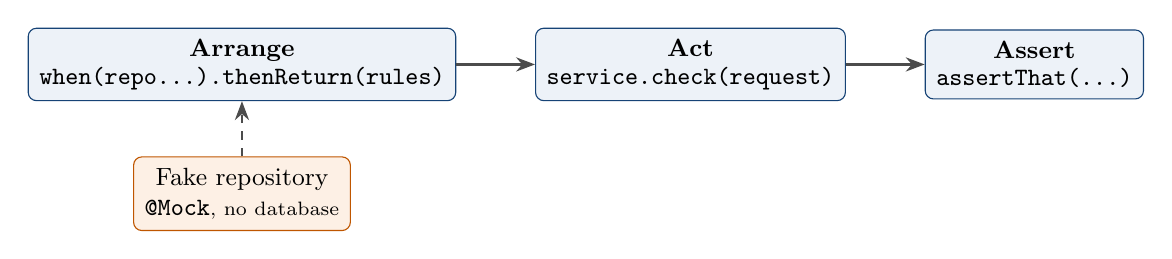
\begin{tikzpicture}[node distance=10mm]
  \node[box] (arr) {\textbf{Arrange}\\[-1pt]{\scriptsize \code{when(repo...).thenReturn(rules)}}};
  \node[box, right=of arr] (act) {\textbf{Act}\\[-1pt]{\scriptsize \code{service.check(request)}}};
  \node[box, right=of act] (ass) {\textbf{Assert}\\[-1pt]{\scriptsize \code{assertThat(...)}}};
  \draw[arr] (arr) -- (act);
  \draw[arr] (act) -- (ass);
  \node[warnbox, below=7mm of arr] (mock) {Fake repository\\{\scriptsize \code{@Mock}, no database}};
  \draw[arr, dashed] (mock) -- (arr);
\end{tikzpicture}
\end{center}

\begin{tabular}{@{}p{5.4cm}p{3.9cm}p{1.9cm}p{3.6cm}@{}}
\toprule
\textbf{Test} & \textbf{Rules the fake returns} & \textbf{allowed} & \textbf{reason} \\
\midrule
\code{noRules\_isDeniedByDefault} & none & false & no matching rule \\
\code{onlyAllowRule\_isAllowed} & ALLOW & true & allowed by policy \\
\code{onlyDenyRule\_isDenied} & DENY & false & denied by policy \\
\code{allowThenDeny\_denyWins} & ALLOW, DENY & false & denied by policy \\
\code{denyThenAllow\_denyWins} & DENY, ALLOW & false & denied by policy \\
\bottomrule
\end{tabular}

\textbf{Lessons}
\begin{itemize}
  \item A method without \code{@Test} is \emph{silently skipped}. Two tests were green but never ran. Always check the count: \code{Tests run: 5}.
  \item The reversed-order test proves the result does not depend on the order of rows. It would catch the old ``return on the first row'' bug.
  \item You cannot write \code{new PolicyRepository()}: it is an interface with about 40 inherited methods. \code{@Mock} is the short way to get a fake.
\end{itemize}

% ------------------------------------------------------------------
\section{Caffeine cache}

\code{check} runs on every agent action, so repeated questions are answered from memory.
The cache is \textbf{not} Redis: it lives inside the Java process (fastest, no network),
and Redis is kept for the Budget Service and the Gateway rate limit.

\begin{center}
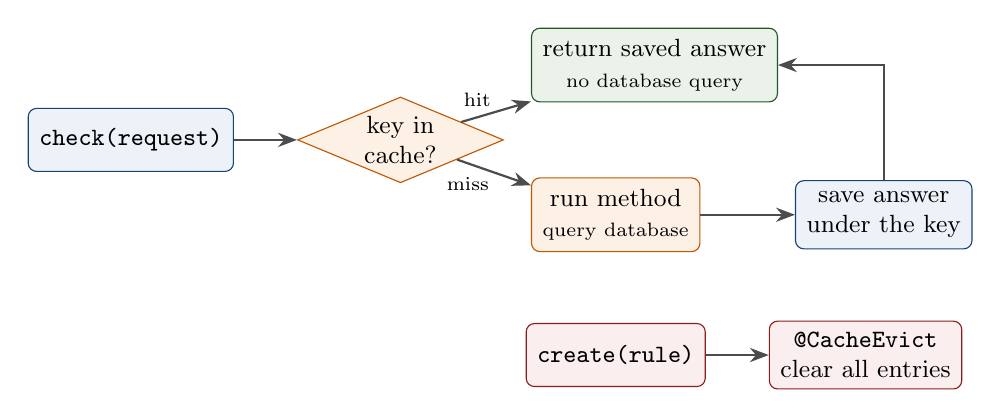
\begin{tikzpicture}[node distance=7mm and 8mm]
  \node[box] (call) {\code{check(request)}};
  \node[dbox, right=of call] (hit) {key in\\cache?};
  \node[okbox, above right=2mm and 10mm of hit] (ret) {return saved answer\\{\scriptsize no database query}};
  \node[warnbox, below right=2mm and 10mm of hit] (db) {run method\\{\scriptsize query database}};
  \node[box, right=12mm of db] (save) {save answer\\under the key};

  \draw[arr] (call) -- (hit);
  \draw[arr] (hit) -- node[lbl,above left] {hit} (ret);
  \draw[arr] (hit) -- node[lbl,below left] {miss} (db);
  \draw[arr] (db) -- (save);
  \draw[arr] (save) |- ($(ret.east)+(0.0,-0.0)$);

  \node[badbox, below=9mm of db] (create) {\code{create(rule)}};
  \node[badbox, right=8mm of create] (evict) {\code{@CacheEvict}\\clear all entries};
  \draw[arr] (create) -- (evict);
\end{tikzpicture}
\end{center}

\begin{lstlisting}
@Cacheable("policyChecks")                                  // on check()
@CacheEvict(value = "policyChecks", allEntries = true)      // on create()
\end{lstlisting}

\begin{tabular}{@{}p{3.6cm}p{12.2cm}@{}}
\toprule
\textbf{Cache name} & \code{"policyChecks"} is a label for the \emph{whole} cache (a map with many entries), not one entry. \\
\textbf{Key} & One parameter $\Rightarrow$ the parameter itself (the \code{CheckRequest} record). Records compare by value, so equal requests share one entry. \\
\textbf{Value} & What the method returned (\code{CheckResponse}). \\
\textbf{Shared?} & By everyone who calls this app instance. The key is the \emph{question}, not the caller. \code{tenantId} is in the key, so tenants never mix. \\
\textbf{\code{allEntries}} & Clears every entry. Needed because \code{create} receives a \code{CreatePolicyRequest}, which never matches a \code{CheckRequest} key. \\
\textbf{Limits} & \code{maximumSize=1000}, \code{expireAfterWrite=60s} (safety net). \\
\bottomrule
\end{tabular}

\textbf{Measured with SQL logging} (number of \code{SELECT} queries on \code{policies}):

\begin{center}
\begin{tabular}{@{}llc@{}}
\toprule
\textbf{Step} & \textbf{Result} & \textbf{Total SELECTs} \\
\midrule
1. first check & false (miss) & 1 \\
2. same check & false (hit) & 1 \\
3. same check & false (hit) & 1 \\
\emph{create an ALLOW rule} & cache cleared & \\
4. check again & \textbf{true} (miss) & 2 \\
5. same check & true (hit) & 2 \\
\bottomrule
\end{tabular}
\end{center}

\textbf{Limits to remember}
\begin{itemize}
  \item Each running copy has its \emph{own} cache. A \code{create} on copy 1 does not clear copy 2, so copy 2 can be stale for up to 60 s. Fix later with Redis or Kafka invalidation.
  \item If 100 requests miss the same new key at once, all may query the database (stampede). \code{sync = true} makes one fetch while the rest wait.
  \item Like \code{@Transactional}, it works through a proxy: calling the method from the same class skips the cache.
  \item The same cache name must be used in \code{@Cacheable} and \code{@CacheEvict}; a typo leaves stale answers.
\end{itemize}

% ------------------------------------------------------------------
\section{\texttt{@Transactional(readOnly = true)}}

Used on \code{check} and \code{list}, which only read.

\begin{tabular}{@{}p{4.2cm}p{11.6cm}@{}}
\toprule
\textbf{Benefit} & \textbf{Why} \\
\midrule
Faster & Hibernate skips the dirty check and flush at the end. \\
Safer & The database connection is read only, so an accidental write is rejected. \\
Consistent & All reads in the method see one view of the data. \\
Clear & The reader sees at once that the method changes nothing. \\
\bottomrule
\end{tabular}

\code{create} writes, so it uses plain \code{@Transactional}. It is a hint, not a lock.

% ------------------------------------------------------------------
\section{DAO and git}

\begin{itemize}
  \item \textbf{DAO} (Data Access Object) hides database code behind an interface. In Spring Data, a \emph{repository is the DAO}, and Spring writes the implementation. A hand-written \code{dao/} class is for custom access, like the Redis Lua script in Week 3.
  \item \textbf{\code{CLAUDE.md}} is no longer tracked: \code{git rm --cached CLAUDE.md} plus a \code{.gitignore} entry. The file stays on disk. The first (already pushed) commit still contains it in history.
\end{itemize}

% ------------------------------------------------------------------
\section{Week 1 checklist}

\begin{center}
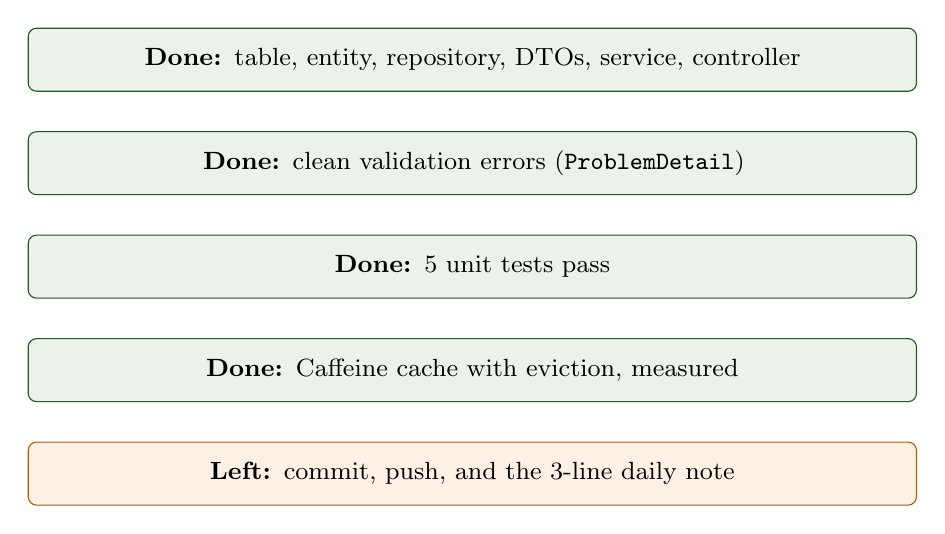
\begin{tikzpicture}[node distance=5mm]
  \node[okbox, text width=11cm] (a) {\textbf{Done:} table, entity, repository, DTOs, service, controller};
  \node[okbox, below=of a, text width=11cm] (b) {\textbf{Done:} clean validation errors (\code{ProblemDetail})};
  \node[okbox, below=of b, text width=11cm] (c) {\textbf{Done:} 5 unit tests pass};
  \node[okbox, below=of c, text width=11cm] (d) {\textbf{Done:} Caffeine cache with eviction, measured};
  \node[warnbox, below=of d, text width=11cm] (e) {\textbf{Left:} commit, push, and the 3-line daily note};
\end{tikzpicture}
\end{center}

\textbf{Interview answers from today}
\begin{enumerate}
  \item \emph{How do you handle validation errors?} ``\code{@Valid} checks the DTO before the controller runs. A \code{@RestControllerAdvice} turns the exception into a standard \code{ProblemDetail} 400 that lists each bad field.''
  \item \emph{How do you test the service without a database?} ``Constructor injection lets me pass a Mockito fake repository, so I test the allow/deny logic alone, including that DENY wins in either order.''
  \item \emph{How does your cache stay correct?} ``Policy checks are cached by request in Caffeine. Creating a rule clears the cache, and entries expire after 60 seconds. With several instances I would use Redis or Kafka invalidation.''
\end{enumerate}

\end{document}
